\section{Model-Free Control}
In this section we will see how to \emph{optimize} the value function of an \emph{unknown} MDP.

Before going into details, there's an important distinction we must make to understand everything that will come after:
\begin{itemize}
    \item \textbf{On-policy} learning: we have some policy $\pi$, we follow this policy, and we learn about it in the process
    \item \textbf{Off-policy} learning: we learn about a policy $\pi$ from experience sampled from an external policy $\mu$ (ex. learning from human behavior)
\end{itemize}

The main framework we are going to use is the same one we saw some sections ago, and that is \emph{policy iteration} in which we alternate two different processes:
\begin{itemize}
    \item \textbf{Policy evaluation:} where we estimate $v_\pi$ (e.g. iterative policy evaluation)
    \item \textbf{Policy improvement:} where we generate a new policy $\pi' \geq \pi$ (e.g. Greedy policy improvement)
\end{itemize}

The question now becomes the following: what can we slot in for these two processes? Firstly we can try to put in Monte-Carlo policy evaluation and $\epsilon$-greedy policy improvement.

\begin{figure}[htbp]
    \centering
    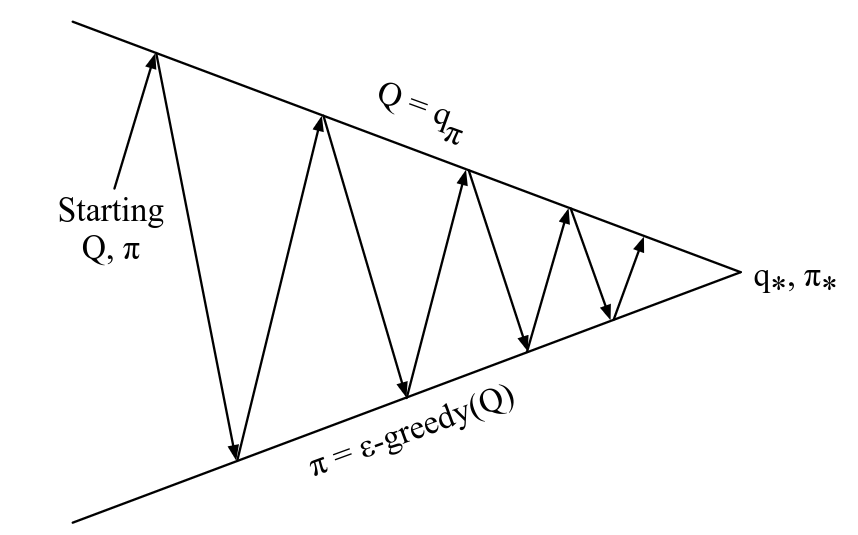
\includegraphics[width=0.5\textwidth]{figures/mc_policy_iteration.png}
\end{figure}

Here we use the $Q$ values because greedy policy improvement over $V$ requires the MDP:
\[
    \pi'(s) = \argmax_{a \in \mathcal{A}} \, \mathbb{E}[\underbrace{R_{t+1} + \gamma V(S_{t+1})}_{\text{Require MDP model}} \mid S_t = s, A_t = a]
\]

Meanwhile, with $Q(s,a)$ the greedy policy improvement becomes \textbf{model-free}:
\[
    \pi' = \argmax_{a \in \mathcal{A}} \, Q(s,a)
\]

Now let's try making this more efficient. We know from DP that in this policy iteration frameworks it is not necessary to go all the way to the top of the $Q=q_\pi$ line every time.

The idea here is to update $Q$ using only a few steps or a single episode, and then immediately update policy $\pi$ to be $\epsilon$-greedy with respect to the current $Q$. This is done because even a slightly better $Q$ gives us a better policy, and a better policy helps us collect better data to refine $Q$.

\begin{figure}[htbp]
    \centering
    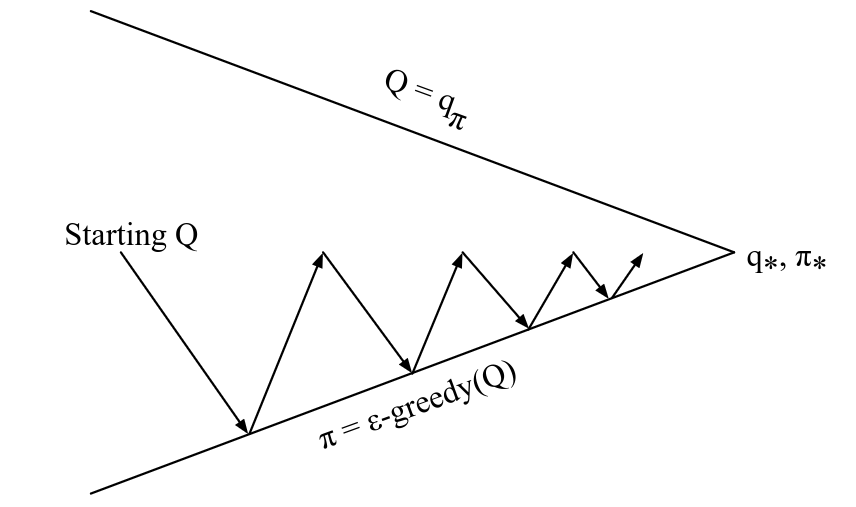
\includegraphics[width=0.5\textwidth]{figures/mc_control.png}
\end{figure}

Now a question comes up: can we guarantee that we will asintotically converge towards the optimal $q_\star$ and $\pi_\star$?

\paragraph{Greedy in the Limit with Infinite Exploration (GLIE)}

\begin{itemize}
    \item All state-action pairs are explored infinitely many times:
        \[ \lim_{k \to \infty} N_k(s,a) = \infty \]
    \item The policy converges on a greedy policy:
    \[
        \lim_{k \to \infty} \pi_k (a \mid s) = \mathbbm{1}\left(a = \argmax_{a' \in \mathcal{A}} \, Q_k(s,a')\right)
    \]
\end{itemize}

\paragraph{GLIE Monte-Carlo Control}
\begin{itemize}
    \item Sample $k$-th episode using our currently policy $\pi: \{ S_1, A_1, R_2, \dots, S_T \} \sim \pi$
    \item For each state $S_t$ and action $A_t$ in the episode:
    \begin{align*}
        N(S_t, A_t) &\gets N(S_t, A_t) + 1 \\
        Q(S_t, A_t) &\gets Q(S_t, A_t) + \frac{1}{N(S_t, A_t)}(G_t - Q(S_t, A_t))
    \end{align*}
    \item Improve policy based on new action-value function:
    \begin{align*}
        \epsilon &\gets 1/k \\
        \pi &\gets \epsilon\text{-greedy}(Q)
    \end{align*}
\end{itemize}

\begin{theorem}
    GLIE Monte-Carlo control converges to the optimal action-value function $$Q(s,a) \to q_\star(s,a)$$
\end{theorem}

\subsection{SARSA: On-policy TD Control}
We already know, in fact, that MC has several disadvantages when compared to TD (such as higher variance, being offline and having to complete the sequence to learn), so the natural idea becomes to substitute MC with TD in the control loop by:
\begin{itemize}
    \item Applying TD to $Q(S,A)$
    \item Use $\epsilon$-greedy policy improvement
    \item Update every time step
\end{itemize}

The name SARSA comes out because of how this algorithm works:
\begin{enumerate}
    \item We start from some state-action pair $(S_t, A_t)$
    \item We then randomly sample from the environment, get a reward $R_{t+1}$ and end up in some state $S_{t+1}$
    \item Then we sample our policy again to generate $A_{t+1}$ from $S_{t+1}$
\end{enumerate}

This rule uses every element of the quintuple of events, $(S_t, A_t , R_{t+1} , S_{t+1} , A_{t+1} )$, that make up a transition from one state-action pair to the next. 

SARSA mainly indicates a particular upgrade rule:
\[
    Q(S_t,A_t) \gets Q(S_t,A_t) + \alpha (R_{t+1} + \gamma Q(S_{t+1},A_{t+1}) - Q(S_t,A_t))
\]

\begin{algorithm}
    \caption{SARSA for On-Policy Control}
    \begin{algorithmic}[1]
        \State Initialize $Q(s,a)$ lookup table $\forall s \in \mathcal{S}, a \in \mathcal{A}$ arbitrarily
        \Repeat{ for each episode}
            \State Initialize $S$
            \State Choose $A$ from $S$ using policy derived from $Q$ (e.g. $\epsilon$-greedy)
            \For{\textbf{each} step of episode}
                \State Take action $A$ and observe $R,S'$
                \State Choose $A'$ from $S'$ using policy derived from $Q$
                \State $Q(S,A) \gets Q(S,A) + \alpha [R + \gamma Q(S',A') - Q(S,A)]$
                \State $S \gets S'$; $A \gets A'$;
            \EndFor
        \Until{$S$ is terminal}
    \end{algorithmic}
\end{algorithm}

\begin{theorem}
    SARSA converges to the optimal action-value function $Q(s,a) \to q_\star(s,a)$ under the following conditions:
    \begin{itemize}
        \item GLIE sequence of policies $\pi_t(a \mid s)$
        \item Robbins-Monro sequence of step-sizes $\alpha_t$:
        \begin{align*}
            \sum_{t=1}^{\infty} \alpha_t = \infty \\
            \sum_{t=1}^{\infty} \alpha_t^2 < \infty
        \end{align*}
        Step sizes must be sufficiently large that we can move $Q$ value as far as we want but eventually changes to $Q$ values vanish
    \end{itemize}
\end{theorem}

\subsection{Q-Learning: Off-Policy TD Control}
In off-policy learning we want to go ahead and evaluate the target policy $\pi(a \mid s)$ while following another behavior policy $\mu(a \mid s)$.

In this case, the learned action-value function, $Q$, directly approximates $q_\star$ , the optimal
action-value function, independent of the policy being followed.

\[
    Q(S_t, A_t) \gets Q(S_t, A_t) + \alpha \left[ R_{t+1} + \gamma \max_a Q(S_{t+1}, a) - Q(S_t, A_t) \right]
\]

Essentially we have the following situation:
\begin{itemize}
    \item The next action is chosen by using the behavior policy: $A_{t+1} \sim \mu(\cdot \mid S_{t+1})$ which, in Q-learning's case, is the $\epsilon$-greedy policy
    \item But we also consider an alternative successor action $A' \sim \pi(\cdot \mid S_{t+1})$ which, in Q-learning's case, is the \textbf{greedy policy}: $\pi(S_{t+1}) = \argmax_{a'} Q(S_{t+1}, a')$
\end{itemize}

What we want to do is to learn a greedy behavior, but we're following some exploratory behavior.

\begin{algorithm}
    \caption{Q-learning (Off-Policy TD Control)}
    \begin{algorithmic}[1]
        \State Initialize $Q(s,a)$ lookup table $\forall s \in \mathcal{S}^+, a \in \mathcal{A}(s)$ arbitrarily, except $Q(\text{terminal}, \cdot) = 0$
        \Repeat{ for each episode}
            \State Initialize $S$
            \For{\textbf{each} step of episode}
                \State Choose $A$ from $S$ using policy derived from $Q$ (e.g. $\epsilon$-greedy)
                \State Take action $A$ and observe $R, S'$
                \State $Q(S,A) \gets Q(S,A) + \alpha \left[ R + \gamma \max_{a} Q(S',a) - Q(S,A) \right]$
                \State $S \gets S'$
            \EndFor
        \Until{$S$ is terminal}
    \end{algorithmic}
\end{algorithm}

\subsubsection{Double Q-Learning}
In Q-learning the target policy is the greedy policy given the current action values, which is defined with a max. In this algorithm, a maximum over estimated values is used implicitly as an estimate of the
maximum value, which can lead to a significant positive bias. 

To better understand this let's use a roulette as an example. Imagine you walk into a casino and sit down at a table. You have two choices:
\begin{itemize}
    \item Choice A (Walk Away): You don't play. You get \$0
    \item Choice B (Play Roulette): You bet \$1 on one of the 36 betting options on the roulette wheel.
\end{itemize}
Because the house always has an edge, the true expected return for placing a roulette bet is slightly negative -- say, $-0.05$ on average, but because roulette is stochastic, you won't get $-0.05$ every single spin. It's natural that we will lose most of the time, but when we get lucky and win, we'll get a positive reward and Q-learning just cares about this max, and nothing else. Because the $\max$ operator always selects the luckiest outlier, Q-learning falls into the illusion that playing roulette is profitable. It will repeatedly choose to play roulette instead of walking away.

The root cause of maximization bias is using the same set of Q-values for both:
\begin{enumerate}
    \item Selecting which action is best ($\argmax_a$)\footnote{Recall that $\max_a Q(S_{t+1}, a) = Q(S_{t+1}, \argmax_a Q(S_{t+1},a))$}
    \item Evaluating the value of that action ($Q(s, a)$).
\end{enumerate}

In general: 
\[
    \mathbb{E}\big[\max_a Q_t(a)\big] \;\geq\; \max_a\, \mathbb{E}\big[Q_t(a)\big] = \max_a q_\star(a)
\]


Double Q-Learning solves this by decoupling action selection from action evaluation using two independent Q-tables ($Q_1$ and $Q_2$). With $p = 0.5$, update $Q_1$ using $Q_2$ for evaluation:

$$Q_1(S_t,A_t) \gets Q_1(S_t,A_t) + \alpha [R_{t+1} + \gamma Q_2(S_{t+1}, \argmax_a Q_1(S_{t+1},a)) - Q_1(S_t,A_t)]$$ 

and otherwise, symmetrically, update Q2 using Q1. The two tables take turns being "the selector" and "the judge," which is what prevents either one from ever grading its own optimistic homework.

We maintain two separate action-value functions, $Q_1(s, a)$ and $Q_2(s, a)$, trained on different subsets of experience (e.g., by randomly splitting incoming time steps) and, when updating:
\begin{itemize}
    \item We use $Q_1$ to \textbf{select} the best action $a^\star = \argmax_a Q_1(S_{t+1},a)$
    \item We use $Q_2$ to \textbf{evaluate} that action $Q_2(S_{t+1}, a^\star)$
\end{itemize}

Going back to the roulette example, Double Q-Learning fixes the maximization bias problem because:
\begin{itemize}
    \item $Q_1$ picks the winner: $Q_1$ looks at its data and picks the highest estimate: "Bet 3 looks best to me!"
    \item $Q_2$ evaluates that pick: Instead of trusting $Q_1$'s positive score, we look up Bet 3 in $Q_2$'s independent dataset.
\end{itemize}

In $Q_2$'s independent history, Bet 3 wasn't as lucky, so the reward turns out as negative.

$$\text{Double Q Target} = Q_2(\text{argmax } Q_1) = Q_2(\text{Bet 3}) = \textbf{Negative value} $$


\subsection{Importance Sampling Corrections}
Firstly we need to estimate the expectation of $f(X)$ under a different (target) distribution $P$:

\begin{align*}
    \mathbb{E}_{X \sim P}[f(X)] &= \sum P(X)f(X) \\
                                &= \sum Q(X) \frac{P(X)}{Q(X)}f(X) \\
                                &= \mathbb{E}_{X \sim Q}\left[ \frac{P(X)}{Q(X)}f(X) \right]
\end{align*}

\subsubsection{Importance Sampling for Off-Policy MC}
The goal is to estimate $v_\pi$ by using returns generated from the behavioral policy $\mu$ to evaluate $\pi$. The key insight is to weight the return $G_t$ according to the similarities between policies $\pi/\mu$:

\[
    G_t^{\pi/\mu} = \left( \frac{\pi(A_t \mid S_t)}{\mu(A_t \mid S_t)} \cdot \frac{\pi(A_{t+1} \mid S_{t+1})}{\mu(A_{t+1} \mid S_{t+1})} \cdot \dots \cdot \frac{\pi(A_T \mid S_T)}{\mu(A_T \mid S_T)} \right) \cdot G_t
\]

For every single step in the episode from $t$ to $T$, you multiply by the ratio:

$$\frac{\text{Probability of taking action } A_t \text{ under target policy } \pi}{\text{Probability of taking action } A_t \text{ under behavior policy } \mu}$$

When policy $\mu$ generates a trajectory, the actions it took might be very likely or unlikely under policy $\pi$. The ratio adjusts for this:

\begin{itemize}
    \item If $\pi(A\vert{}S) > \mu(A\vert{}S)$: policy $\pi$ would have taken this action much more often than $\mu$ did. Therefore, this episode's return $G_t$ was under-represented, so we up-weight it.
    \item If $\pi(A\vert{}S) < \mu(A\vert{}S)$: policy $\pi$ rarely takes this action compared to $\mu$. This return was over-represented, so we down-weight it.
    \item If $\pi(A\vert{}S) = 0$: Policy $\pi$ would never take this action. The entire return $G_t$ gets zeroed out because it's irrelevant to $\pi$.
\end{itemize}

Multiplying together $\pi(A_t|S_t)/\mu(A_t|S_t)$ across an entire episode means the correction weight is a product of ratios, one per timestep. Even if each ratio is well-behaved, the product's variance can grow exponentially with episode length. This is why full-return importance sampling is rarely used in practice for long episodes, and why the TD version in \ref{sec:importance_sampling_td} (which only needs a single step's ratio per update) is generally preferred. Note also that this only works if $\mu(a \mid s) > 0 $, otherwise we'd have $0$ in the denominator.

\subsubsection{Importance Sampling for Off-Policy TD}\label{sec:importance_sampling_td}
Here we use the TD targets generated from $\mu$ to evaluate $\pi$ and weigh them by importance sampling:

\[
    V(S_t) \gets V(S_t) + \alpha \left( \frac{\pi(A_t \vert S_t)}{\mu(A_t \vert S_t)}(R_{t+1} + \gamma V(S_{t+1})) - V(S_t) \right)
\]

\subsection{Expected SARSA}
Consider the learning algorithm that is just like Q-learning except that instead of the maximum over next state-action pairs it uses the expected value, taking into account how likely each action is under the current policy. That is, consider the algorithm with the update rule:

\begin{align*}
    Q(S_t, A_t) &\gets Q(S_t, A_t) + \alpha \left[ R_{t+1} + \gamma \mathbb{E}_\pi [Q(S_{t+1},A_{t+1}) \mid S_{t+1}] - Q(S_t, A_t) \right] \\
               &= Q(S_t, A_t) + \alpha \left[ R_{t+1} + \gamma  \sum_{a} \pi(a \mid S_{t+1})Q(S_{t+1},a) - Q(S_t, A_t) \right]
\end{align*}

Given the next state, $S_{t+1}$, this algorithm moves \emph{deterministically} towards the same direction as SARSA moves \emph{in expectation}, and accordingly it is called \emph{Expected SARSA}. Thus, expected SARSA eliminates the variance caused by random action selection ($A_{t+1}$). Note that the cost of this variance reduction is computational: the sum over all actions costs $\mathcal{O}(\lvert A \rvert)$ per step, versus $\mathcal{O}(1)$ for plain SARSA or Q-learning.

Expected SARSA can be both On- and Off-Policy:
\begin{itemize}
    \item If we take $\pi$ as the greedy policy ($\pi(a \mid S_{t+1}) = 1$ for the best action, $0$ otherwise), then Expected SARSA collapses into standard Q-learning.
\end{itemize}

\begin{table}[h]
    \centering
    \caption{On-Policy vs.\ Off-Policy Control Algorithms}
    \begin{tabularx}{\linewidth}{l l l X}
    \toprule
    \textbf{Algorithm} & \textbf{On/Off-policy} & \textbf{Update target} & \textbf{Notes} \\
    \midrule
    SARSA & On-policy & $R + \gamma Q(S',A')$, $A'$ & Learns the value of the $\epsilon$-greedy policy it runs \\
    \addlinespace
    Q-Learning & Off-policy & $R + \gamma \max_a Q(S',a)$ & Prone to maximization bias \\
    \addlinespace
    Double Q-Learning & Off-policy & $R + \gamma\, Q_2\!\left(S', \operatorname*{argmax}_a Q_1(S',a)\right)$ & Decouples selection from evaluation \\
    \addlinespace
    Expected SARSA & Either & $R + \gamma \sum_a \pi(a\mid S')Q(S',a)$ & Reduces to Q-learning if $\pi$ is greedy \\
    \addlinespace
    Off-policy MC (IS) & Off-policy & episode return weighted $\prod \pi/\mu$ & High variance \\
    \bottomrule
    \end{tabularx}
\end{table}